\subsection{Stability}

If a body in \textbf{stable equilibrium} is displaced then released, it \underline{returns to its equilibrium position}. E.g. a clothes hanger hanging from a support swings back to its equilibrium position.
\begin{enumerate}
    \item The \textbf{centre of mass} of the object is directly below the point of support when the object is at rest.
    \item The \textbf{weight of the object} is considered to act at its centre of mass.
    \item Thus the support force and the weight are \underline{directly equal and opposite to each other} when the object is in equilibrium.
    \item When the object is displaced, the line of action of the weight no longer passes through the point of support.
    \item So the weight returns the object to equilibrium.
\end{enumerate}

If a body is in \textbf{unstable equilibrium} is displaced slightly, it will experience a force in the direction of displacement (away from equilibrium). E.g. a plank balanced on a drum will roll off the drum when displaced slightly then released.
\begin{enumerate}
    \item The \textbf{centre of mass} of the object is directly above the point of support when it is in equilibrium.
    \item The support force is equal and opposite to the weight.
    \item If displaced slightly, the centre of mass is \textbf{no longer above the point of support}.
    \item The weight will therefore acts to turn it further away from the equilibrium position.
\end{enumerate}

\subsubsection*{Tilting and Toppling}

\textbf{Tilting} is where an object at rest on a surface is acted on by a force that \textbf{raises it up} on one side. To make a bookcase tilt, the force must turn it clockwise about point $P$. The weight of the bookcase provides an anticlockwise moment about $P$.
\begin{center}
    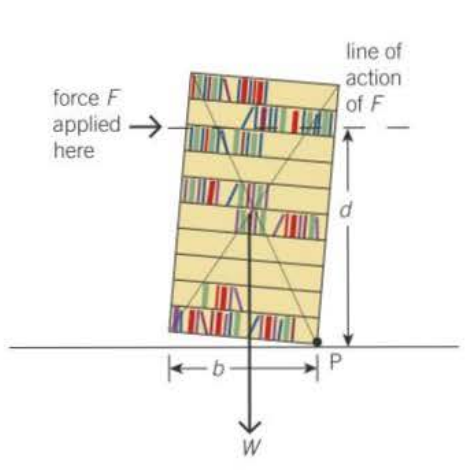
\includegraphics[width=5cm]{img/tilting}
\end{center}
\begin{itemize}
    \item The clockwise moment about of $F$ about $P$ is $Fd$, where $d$ is the perpendicular distance between the line of action of the force and the pivot.
    \item The anticlockwise moment of $W$ about $P$ is $Wb/2$ where $b$ is the width of the bookcase.
\end{itemize}

For tilting to occur
$$Fd>Wb/2$$

A tilted object will \textbf{topple over} if it is tilted too far.
\begin{itemize}
    \item If the object is tilted so much that the line of action of \textbf{its weight passes beyond the pivot}, the object will topple over if allowed to.
    \item The position where \textbf{the line of action of the weight passes through the pivot} is the furthest it can be tilted without toppling.
\end{itemize}
